\chapter{Implementierung}\label{chapter:Implementierung}

\section{Laden der Modelldateien}
Um die Dateien zu laden, die vom Nutzer hochgeladen wurden, mussten drei Klassen implementiert werden. Die \textit{\nameref{sec:model}}-Klasse repräsentiert ein Modell und speichert die relevanten Daten des Modells für das Rendering. Zum Laden der Daten greift es auf die \textit{\nameref{sec:objloader}}-Klasse und die \textit{\nameref{sec:textureloader}}-Klasse zurück.

\subsection{ObjLoader}\label{sec:objloader}
Die \textit{ObjLoader}-Klasse ist dafür zuständig die Daten aus der Obj-Datei des Modells einzulesen und in das passende Format für OpenGL umzuwandeln.\\
Bei ihrer Instanziierung wird der Klasse der Pfad zu der Datei die eingelesen werden soll übergeben.
Nachdem diese geladen wurde, muss die Datei Zeile für Zeile durchlaufen werden und anhand der Abkürzungen, mit denen jede Zeile beginnt, der Datentyp bestimmt werden. \\
Der Aufbau einer Obj-Datei unterliegt dabei dem folgenden Muster (vergleiche dazu auch Abbildung \ref{fig:obj-datei}):\\
Jede Zeile enthält ein Datenobjekt, welches über die die Kennung zu einem bestimmten Datentyp zugeordnet werden kann. 
Zu Beginn der Datei werden alle Einzelteile des Modells definiert:
\begin{description}
\item[Vertex (v):] Ein Vertex repräsentiert einen Eckpunkt des Objektes. Dazu werden in der Zeile die drei Koordinaten des Punktes gespeichert.
\item[Textur (vt):] Diese Zeile besteht aus zwei Koordinaten, welche einen Punkt in einem zweidimensionalen Bild, der Texturdatei, repräsentieren.
\item[Normalenvektor (vn):] Dieser Kennung folgenden die drei Koordinaten eines Normalenvektors  
\end{description}

\begin{figure}
\centering
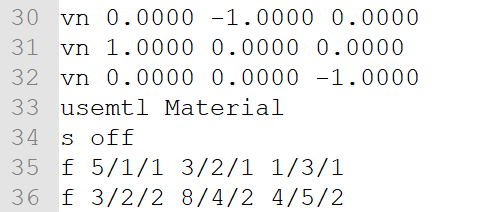
\includegraphics[width=0.6\textwidth]{Abbildungen/obj-datei.png}
\caption[Obj-Dateiformat]{Ausschnitt aus einer Obj-Datei. (Quelle: Eigene Darstellung)}
\label{fig:obj-datei}
\end{figure}
Damit OpenGL mit diesen Einzelteilen arbeiten kann, müssen diese noch zusammengesetzt werden. \\
Die dafür nötigen Informationen speichern die sogenannten Faces (deutsch: \glqq Gesichter\grqq ), welche die Kennung f besitzen. Sie beschreiben die einzelnen Flächen des Modells. Da zuvor im \nameref{chapter:Entwurf}) die Anforderung an die Obj-Dateien gestellt wurde, dass diese tranguliert werden, handelt es sich bei den Flächen immer um Dreiecke. \\ 
Die Zeile eines dieser Dreiecke speichert dafür für jeden Eckpunkt der Fläche drei Indices die auf jeweils einen der  zuvor definierten Vertices, Texturkordinaten und Normalenvektoren verweisen. Dadurch wird neben der Koordinaten der Fläche, auch der zugehörige Ausschnitt der Textur und der Normalenvektor der Datei definiert. \\
Das Programm erstellt aus diesen Daten drei Listen (jeweils eine für Vertices, Texturkoordinaten und Normalenvektoren), indem es für jede Fläche die Daten jedes Punktes an die entsprechende Liste anhängt.\\
Auf diese Listen kann dann über die Klassenvariablen des \textit{ObjLoader}-Objektes zugegriffen werden.

\subsection{TextureLoader}\label{sec:textureloader}
Die \textit{TextureLoader}-Klasse hat die Aufgabe die Textur-Datei einzulesen und OpenGL zur Verfügung zu Stellen. Dazu wird zunächst mit \textit{GLES20.glGenTextures} eine Textur erzeugt und eine Referenz in \textit{textureHandle} gespeichert. Anschließend wird die Texturdatei des Modells als Bitmap an die Textur gebunden und die Filter zur Texturverarbeitung gesetzt. 

\subsection{Model}\label{sec:model}
Die \textit{Model}-Klasse beruht auf dem Grundgerüst von der \textit{Cube}-Klasse, welche ein Teil von ARToolKit ist und einen simplen Würfel darstellt.\\
Diese Klasse wurde im Rahmen der Arbeit so modifiziert, dass sie beliebige Modelle speichern kann.\\
Dazu werden mittels der \textit{\nameref{sec:objloader}}-Klasse die Daten aus der Obj-Datei geladen und in Buffern gespeichert. Des weiteren wird mit Hilfe der \nameref{sec:textureloader}-Klasse die Textur geladen und eine Referenz auf diese erzeugt.\\
Um das Modell zu Rendern verfügt es über eine \textit{draw}-Methode, welche die Daten des Modells an das Shader Programm übergibt.

\section{Augmented Reality}
Die Sturktur, die zur Umsetzung der Augmented Reality genutzt wurde, beruht zum Großteil auf dem Konzepten und Klassen von ARToolKit und wurde dann an die Anforderungen dieser Arbeit angepasst.

\subsection{CameraFragment}
Das \textit{CameraFragment} bildet den Grundbaustein des Augmented Reality Fragments. Es erweitert das \textit{ARFragment}, eine Klasse die im Laufe der Arbeit implementiert wurde. Sie ist von ihrer Funktionalität idententisch zu der \textit{ARActivity}-Klasse von ARToolKit und wurde lediglich an die Anforderungen eines Fragments angepasst, um in das Userinterface eingefügt werden zu können.\\
Zum einen wird in dieser Klasse die in C++ geschriebene, native ARToolKit-Bibliothek geladen, zum anderen dient die Klasse dazu alle wichtigen Objekte zu initialisieren und mit einander zu verbinden.
Dafür wird unter anderem die visuelle Oberfläche in Form eines \textit{FrameLayouts}, welches ein \textit{GLSurfaceView} enthält, auf dem später das Kamerabild, sowie die Modelle projiziert werden, erzeugt.
Des weiteren wird in dieser Klasse der \textit{ARRenderer} an das \textit{ARFragment} gebunden.

\subsection{EducationARRenderer}
Die \textit{EducationARRenderer}-Klasse erweitert ARToolKits \textit{ARRender}. Die Aufgabe des Renderes ist es die AR-Szene zu konfigurieren und die Visualisierung der AR-Modelle einzuleiten. Dazu werden zunächst in der \textit{configureARScene}-Methode die Marker gesetzt. In der \textit{draw}-Funktion werden dann die zuvor definierten Marker getrackt und die Model-, View- und Projektionsmatrix berechnet. Diese Matrizen werden dann an die \textit{draw}-Funktionen des entsprechenden Modells übergeben, um die Modelle mit der richtigen Transformation zu visualisieren.\\

\section{Markergenerierung}
Damit der Nutzer die Modelle nutzen kann, muss die Anwendung dazu in der Lage sein selber Marker zu erzeugen. Dazu wurde die folgende Klasse im Rahmen der Arbeit implementiert. 
\subsection{MarkerGenerator}
Die \textit{MarkerGenerator}-Klasse ist eine Hilfsklasse die über die \textit{generateMarker}-Methode einen Marker mit einer bestimmten ID und Patterngröße $n$, die über die Methodenparameter übergeben werdem, erzeugt. Dazu wird zunächst eine quadratische Bitmap der Größe $n$ x $n$ erzeugt. Anschließend muss aus der übergebenen ID ein Barcodemuster erzeugt werden.
\begin{figure}[h!]
\centering
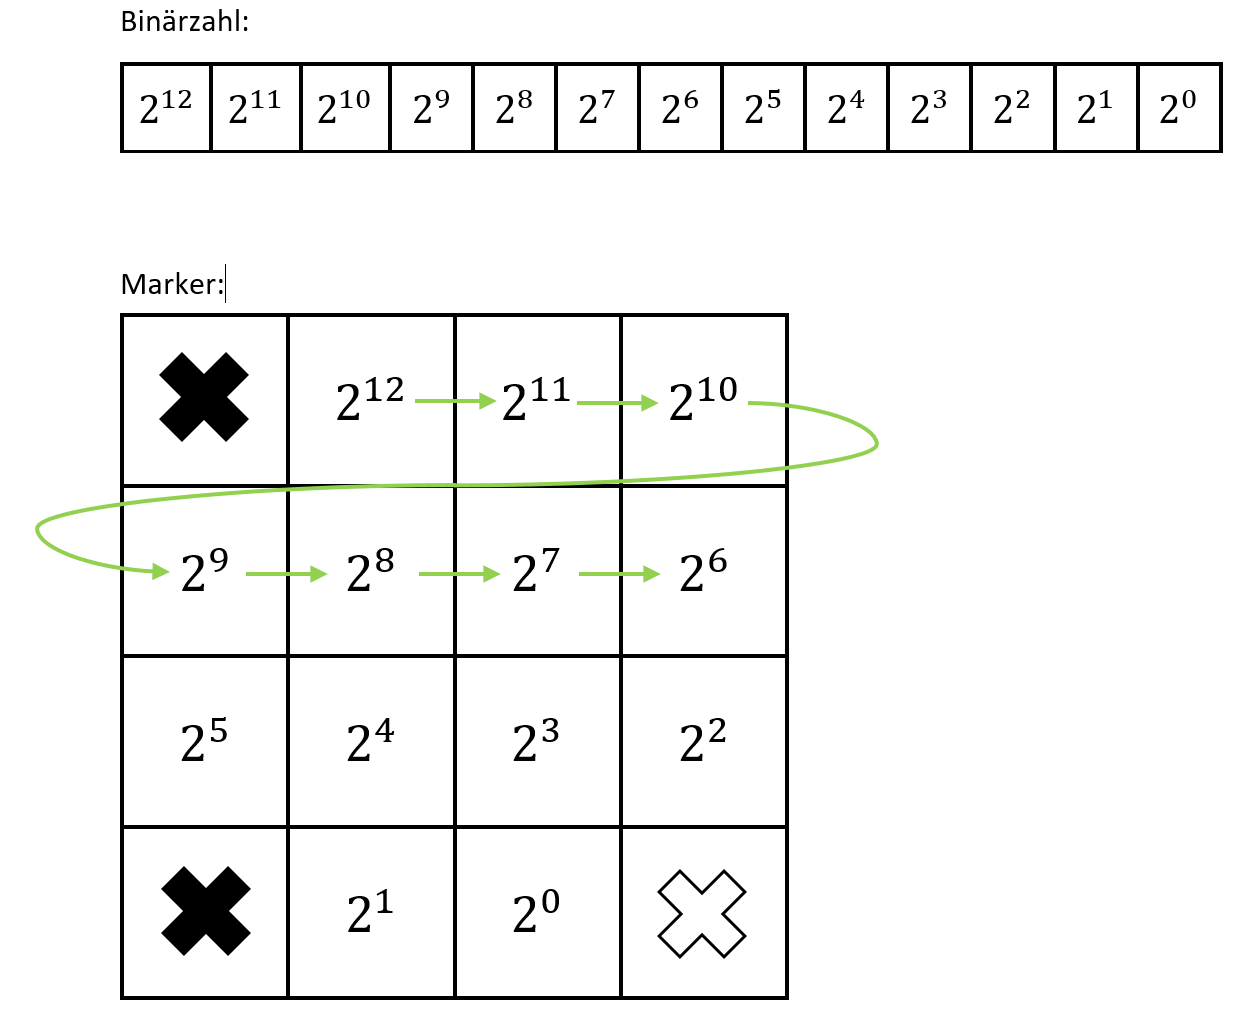
\includegraphics[width=0.8\textwidth]{Abbildungen/barcode-creation.png}
\caption[Markererstellung]{Visualiserung des Vorgehens zur Erstellung eines 4x4 Barcodepatterns. (Quelle: Eigene Darstellung)}
\label{fig:barcode-creation}
\end{figure}\\ 
Dieses geschieht indem die ID zunächst in eine Binärzahl mit der Länge $n^2 - 3$ umgewandelt wird. Jede Null in der Binärzahl repräsentiert ein weißes Feld und jede Eins ein schwarzes Feld im Barcodepattern. Damit das Pattern am Ende jedoch Rotationsinvariant ist sind insgesamt drei Felder des Musters bereits eine feste Farbe zugeordnet(in Abbildung \ref{fig:barcode-creation} durch Kreuze in der entsprechenden Farbe dargestellt). Für diese vordefinierten Felder werden deshalb entweder eine Null oder eine Eins an den entsprechenden Stellen des Strings, der die Binärzahl repräsentiert , eingefügt.\\
Im nächsten Schritt kann dann lediglich die Bitmap durchlaufen werden und der Wert des Strings an der Stelle $i*n + j$ eingefügt werden, wobei i die aktuelle Zeile und j die die aktuelle Spalte repräsentiert. \\ 
Zuletzt muss die Grafik, noch hochskaliert werden, damit diese besser in Dokumente eingefügt werden kann und ein
ein schwarzer Rahmen mit Hilfe der \textit{addBorder}-Methode um das Barcodepattern gezogen werden, um die Anforderungen von ARToolKit zu befriedigen.
